\section*{Neural Network Models}
\label{sec:nn_models}
\addcontentsline{toc}{section}{\nameref{sec:nn_models}}

\subsection{General}
The choice to use neural networks for the final model was multi-faceted.  First, these types of models are very good at capturing complex non-linear interactions.  This appears to be the case with the data set given the failure of lasso models as well as the low percentage of variance capture for the first few dimensions of the principal component and partial least squares analyses.  Secondly, neural networks have the ability to use customized loss functions.  This is beneficial because it is important to highlight practicality of the results returned.  As the estimated energy consumption grows, it is somewhat acceptable for the error rate to grow proportionally if it results in the low estimates to have better error rates using a homoscedastic loss function.  As an example, a large datacenter may use a lot of energy so a slightly higher relative error rate may not be a big issue since it could be a small portion of the overall consumption; however, if a non-heated warehouse with a moderate error rate, comparative to the rest of the data set, would be wildly innacurate.  Therefore, the loss function chosen for this set of models was chosen to be the mean squared logarithmic error in an effort to reflect this reasoning.

\subsection{Hyperparameter Training}
In order to select the most optimized set of parameters, some hyperparameter training was performed.  Some standard searches were made, such as varying the dropout rate, regularization, learning rate, and batch size; however, one additional training set was incorporated to highlight the goals of this study.  A series of models were tested which had an incrementally decreasing number of variables, by least importance, in order to test the loss of accuracy.
\newpage
\subsection{Electricity}
\subsubsection{Summary}
The final selected model consisted of a 3 hidden layers of 300 nodes, using a dropout rate of 0.6, no regularization, batch sizes of 50 and XXX variables for selection.  The number of variables is greatly reduced while maintaining relativively similar performance

\begin{figure}[h]
\centering
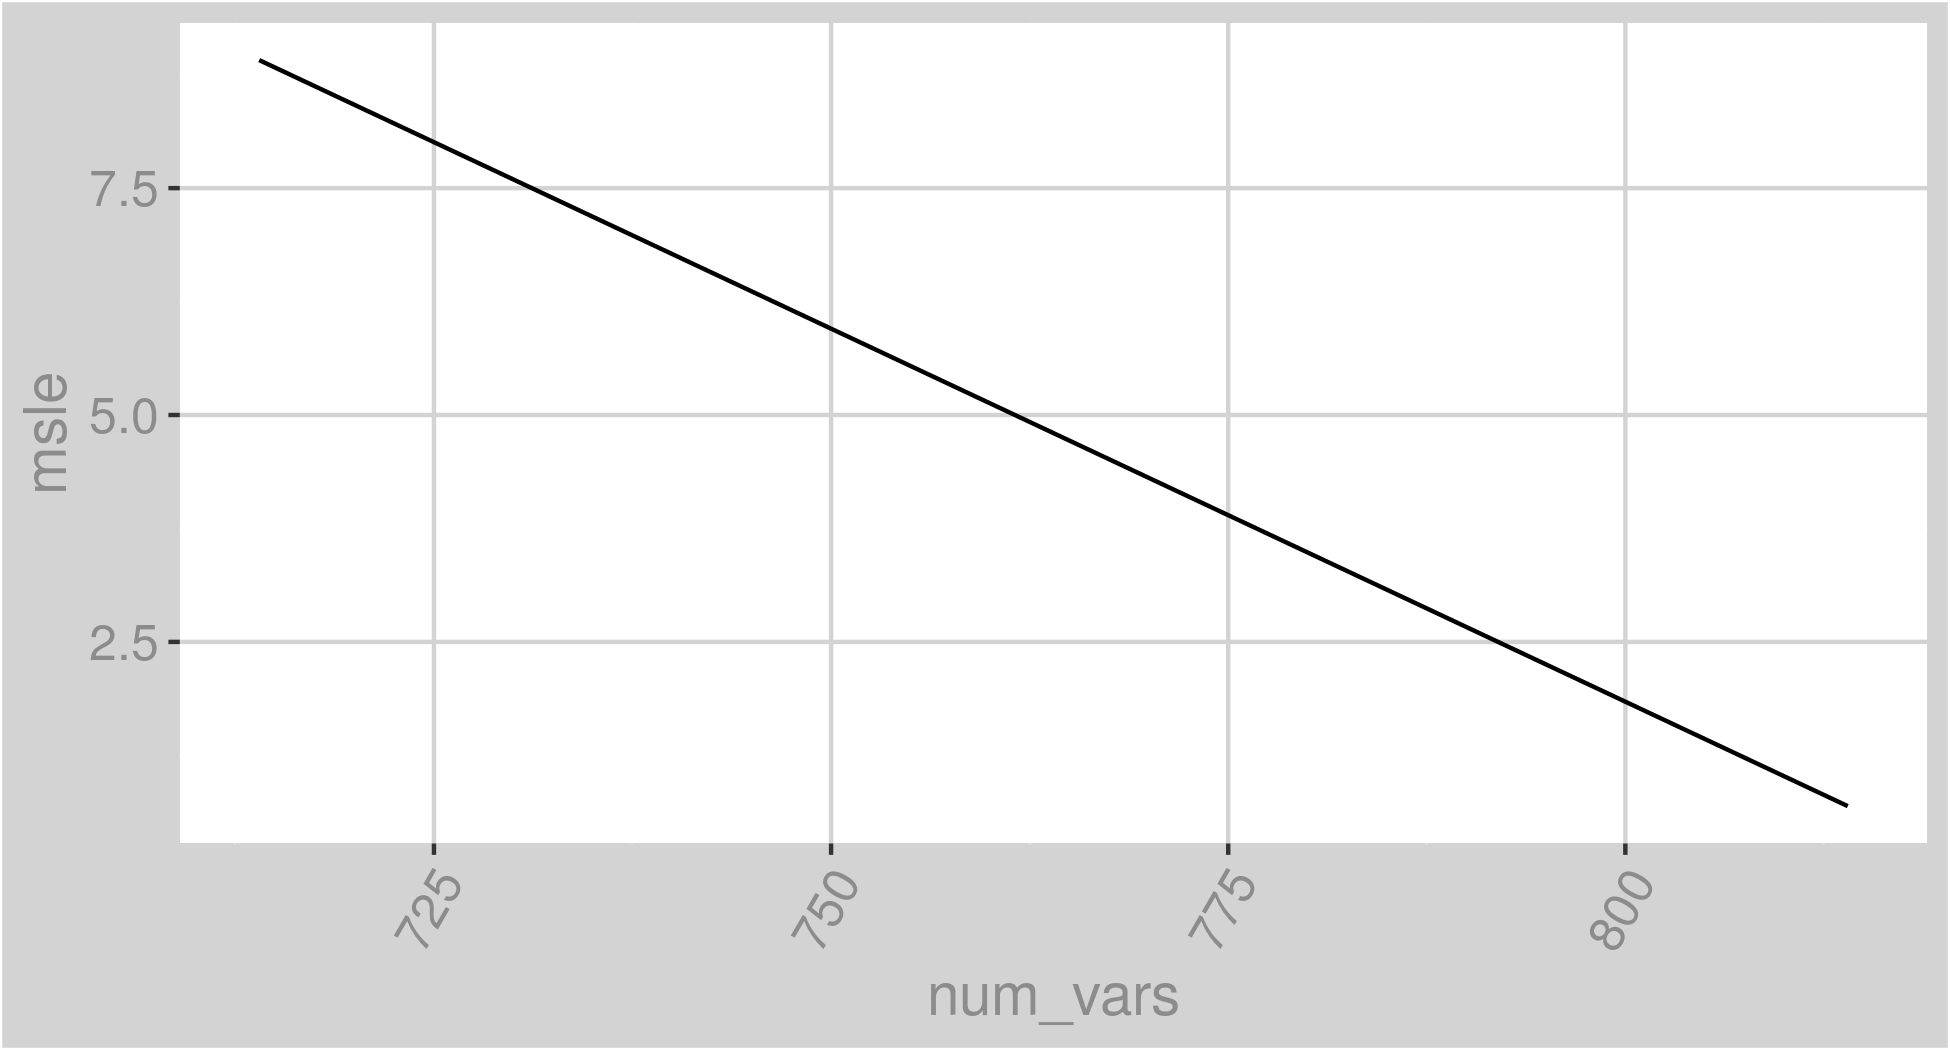
\includegraphics[width=\textwidth, height=0.4\textheight]{Images/electricity_nn_error.png}
\end{figure}

The final selected model has a msle of XXX and mse of XXX.  Comparing this to the previous feature extraction models, which used many more variables, the performance is ....

The resdiuals indicate.... It is noted that the variance scales with the response variable, by design; however, since neural network models do not operate on a principle of homoscedacitity, only underlying patterns are of concern.  

In summary, the resulting predictions appear to be ....  \textit{\hyperref[appendix:electricity:nn_full]{Appendix}}

\subsubsection{Future Work}
While it was determined that some heteroscedacitity would be acceptable, there does appear to be area for improvement.  Additionally, as mentioned at the beginning of this report, the sampling of this data set was stratified to reflect the building population.  However, it is noted that there are some classes that have greater variance than others.  Therefore, it may be useful to use this stratification as a weighted method, based on \lstinline{PBAPLUS}, in order to try and emphasize accuracy on the most prevalent budiding types. 

\FloatBarrier
\newpage
\subsection{Natural Gas}

\FloatBarrier
\newpage
\subsection{District Heat}

\FloatBarrier
\newpage
\subsection{Fuel Oil}